	\chapter{METHODOLOGY}
	\label{chap:methodology}
	
	\section{Vehicle Classification}
	
	 Electric vehicles have been classified primarily into four major categories as shown in Figure~\ref{fig:classification} 
	 	
			\begin{figure}[h]
				\centering
				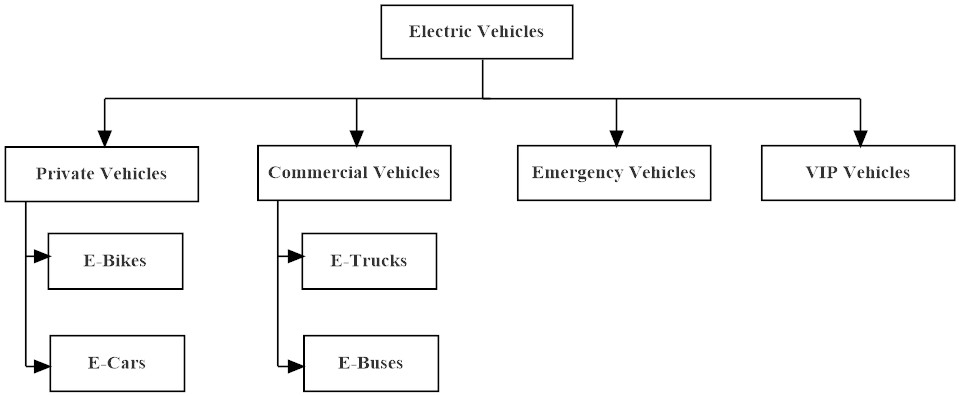
\includegraphics[width=0.7\linewidth]{./Figures/classification}
				\caption{Vehicle Classification}
				\label{fig:classification}
			\end{figure}
		
	The above classification is made by comparing the battery capacity of the vehicles from the data taken with the battery capacity of the similar kind of vehicles in the market.

	\par {Private vehicles are further classified into E-bikes and E-cars with average battery capacity of 400 $Wh$ to 500 $Wh$ and 40 $kWh$ to 100 $kWh$ respectively. Commercial vehicles are classified into E-Truck and E-Bus with an average battery capacity of 100 $kWh$ and 60 to 548 $kWh$ respectively. Emergency vehicles have a battery capacity of around 105 $kWh$ and VIP vehicles have around 90 $kWh$ to 200 $kWh$.
	}
	
	\section{Travel Pattern Establishment}
	
	Travel pattern for three main vehicle subcategories of the above mentioned vehicle categories namely E-car, E-Truck and E-Bus are now taken and travel patterns of the same have been established by using the Battery capacity, Time taken to full charge, Time period of the vehicle when it is connected to the grid , charging rate and discharging rate \cite{evdata}.
	
	Car: ID – 13646 \cite{evdata} is chosen for E-Car as its battery capacity matches with the most common types of E-cars in the market. The
	battery capacity range of this vehicle is 54 $kWh$. The time taken for 100\% charging of battery
	happens to be 1 hour 40 minutes. It then continues to Travel for 6 hour 30 minutes after which the Battery's Charge of the vehicle is depleted. This vehicle is connected to the grid for 5 hours 20 minutes until the next trip. The charging/discharging rate is 10.8 $kW$ per twenty minutes.
	
	Truck: ID – 4428 \cite{evdata} is chosen for E-Truck as its battery capacity matches with the most common types of E-Trucks in the market. The
	battery capacity of this vehicle is 99.2 $kWh$. The time taken for 100\% charging of battery
	happens to be 4 hours. It then continues to Travel for 14 hours after which the Battery's Charge of the vehicle is depleted. This vehicle is connected to the grid for 10 hours until the next trip. The charging/discharging rate is 8.267 $kW$ per twenty minutes.
	
	Bus: Vehicle ID – 16034 \cite{evdata} is chosen for E-bus as its battery capacity matches with the most common types of E-Buses in the market. The
	battery capacity of this vehicle is 199.95 $kWh$. The time taken for 100\% charging of battery
	happens to be 5 hours 20 minutes. It then continues to Travel for 13 hours after which the Battery's Charge of the vehicle is depleted. This vehicle is connected to the grid for 11 hours until the next trip. The charging/discharging rate is 12.5 $kW$ per twenty minutes.
	



	\section{Charging/Discharging pattern Establishment}
	
	A 24 hour time scale is taken for charging/discharging pattern formulation. This time scale is further subdivided into 72 time blocks  because the classified vehicles have different battery
	capacity range. This split up is done to find the best efficient charging/discharging pattern in
	order to reduce the cost that is paid to the grid for the beneficial of consumers.
	
	\section{Flowchart}
	
	1. With the help of the device data calculate the time period T for which the vehicle is
	connected to the grid.
	
	\noindent 2. Calculate SoC threshold,t for every vehicle.
	
	\noindent 3. The SoC residual,t and SoC consumed,t are determined for the time block t
	\noindent 4. The SoC residual,t is compared with SoC threshold,t
	\begin{itemize}


	 \item If the condition is true then the time must be equal peak demand. If it is equal then
	the vehicle stays idle. If the time is not equal to peak demand then it is then
	checked with the real price algorithm and if it satisfies the algorithm ten the
	vehicle goes to charging, if not the vehicle stays idle.
	
	\item If the condition is not true then time is checked with the peak demand and the
	vehicle is given a priority of either 1 or 0. 1 means the vehicle has to charge and if
	0 then the vehicle discharges when the time is equal to peak demand. When t and
	peak demand are not equal the vehicle stays idle.
	
		\end{itemize}
	
	\begin{figure}
		\centering
		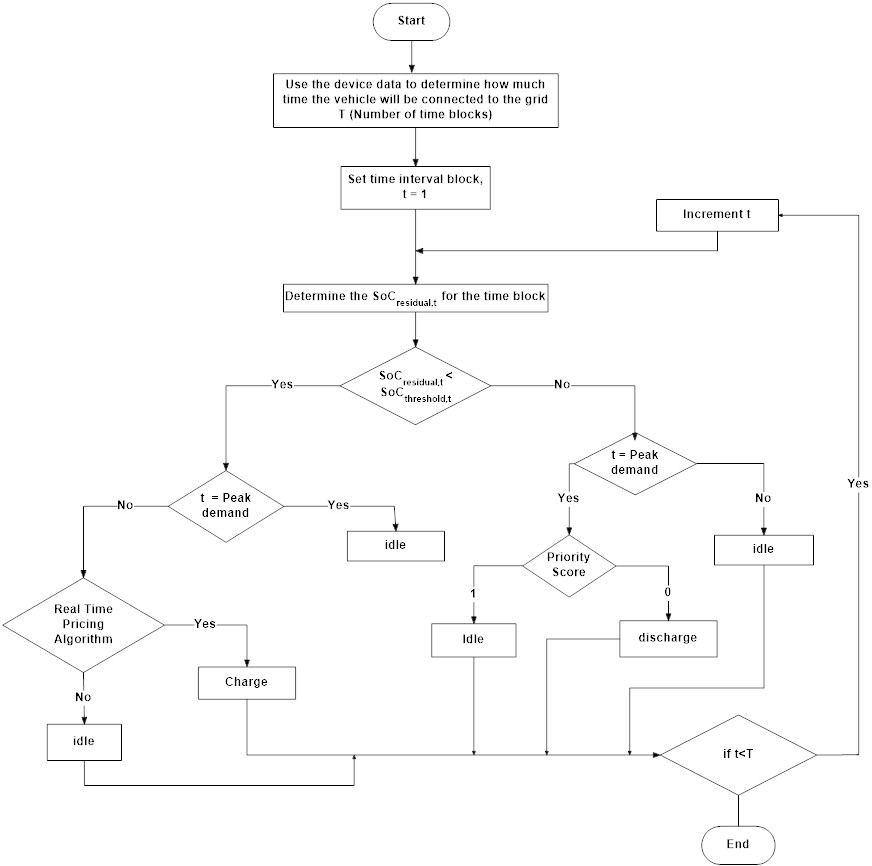
\includegraphics[width=0.9\linewidth]{Figures/Ev_flowchart}
		\caption{}
		\label{fig:evflowchart}
	\end{figure}


	\section{Real Time Price}
	
		\begin{figure}[!h]
			\centering
			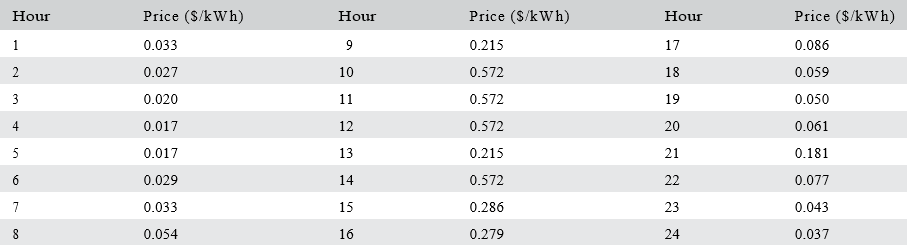
\includegraphics[width=0.7\linewidth]{Figures/rtp}
			\caption{}
			\label{fig:rtp}
		\end{figure}
	
	